\section{Theory}

A polarizing microscope is used for the experiments in this report. In this section the basic principles of a polarizing microscope and the theory that is used for the experiments are described.

\begin{wrapfigure}{r}{0.3\textwidth}
    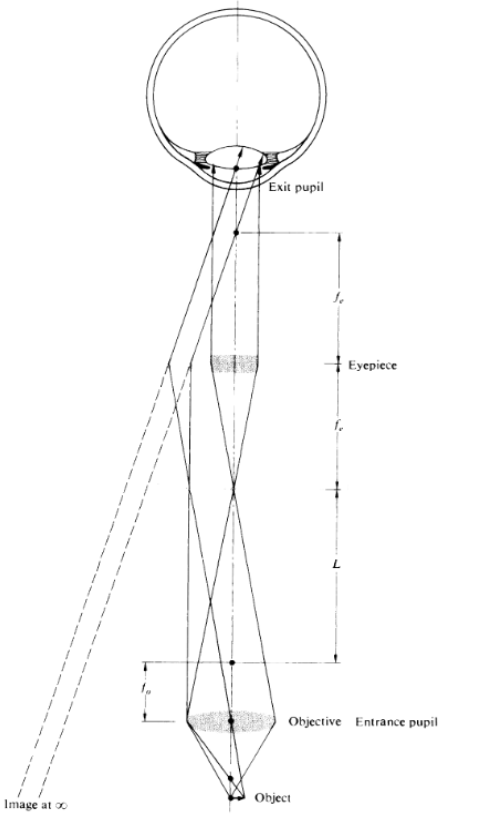
\includegraphics[width=0.25\textwidth]{afbeeldingen/compound_microscope.png}
  	\caption{Schematic drawing of a compound microscope. $f_{e}$ and $f_{o}$ correspond to respectively to the focussing distance of the eyepiece and objective. This figure was apdapted from \cite{hecht}.}
  	\label{fig_compound_microscope}
\end{wrapfigure}

\subsection{Microscopy}


Most modern microscopes are compound microscopes. These type of microscopes can achieve a relatively high angular magnification for nearby objects (\cite{hecht}). For this system, an objective, being the entrance pupil of the system, creates a real inverted, magnified image. The eyepiece creates a virtual images with greater magnification which can be viewed comfortably. The total magnification of the microscope is the product of the individual magnifications of the eyepiece and objective (\cite{hecht}). See figure \ref{fig_compound_microscope} for a schematic drawing of a basic compound microscope.


Polarizing microscopes are a type of microscopes that make use of polarizing windows. A polariser is placed in between the light source and the sample and an analyser is placed after the sample. Since the polariser and analyser block all the light except for one specific light polarization, they allow the viewer to see some of the sample's optical properties such as birefringence. 

The microscope that is used in all experiments is a Leica DM EP microscope. Its manual can be found in appendix \ref{appendix_manual}. This microscope is used in combination with $4\times$, $10\times$, $40\times$ Hi Plan POL objectives with respectfully a 0.10, 0.22 and 0.65 numerical aperture. A color CCD camera in combination with NI Vision Assistant software is used to acquire digital images.

\subsection{size measurements}
In this experiment it was chosen to use a CCD camera to record the imaged from the microscope. To measure distances in a sample it is possible to convert a distance in pixels, $n_{pixels}$, to physical unit such as meters. For this, we need a conversion factor that gives the length in meters per pixel, $l_{pixel}$. The physical distance, $d_{physical}$ can easily be calculated using equation \ref{eq_distance}.

\begin{equation}
	\label{eq_distance}
	d_{physical} = l_{pixel} \cdot n_{pixels}
\end{equation}

The value for $l_{pixel}$ depends on the specifications of the camera but primarily on the magnification of the microscope. The value for $l_{pixel}$ should be larger for greater magnifying power.
\bigskip

One of the purposes of this experiment is to find out if it possible to do microscopic measurements with the given microscope. Human hairs and glass fibres have a diameter in the range of 10 - 100 $\mu m$. Measuring the diameter could give insights into the suitability of the given microscope for measurements of this scale.

Another purpose for a microscope could be to find sizes of many particles. From this information one could get the average particle size and the distribution for these values. Starch particles have a size up to 100 $\mu m$ and are often of elliptical shape (\cite{starch}). The size of ellipse-shaped starch particles will be measured in this experiment. The cross section of a particle, $A$, can be calculated using the major and minor diameter of the ellipse, respectively $a$ and $b$, and equation \ref{eq_ellipse}.

\begin{equation}
	\label{eq_ellipse}
	A = 1/4 \cdot a \cdot b \cdot \pi
\end{equation}
	
\subsection{Birefringence}
Birefringence is a phenomenon that occurs in many materials such as polyethylene, ice and calcite (\cite{hecht}). This optical property arises when the refractive index depends on the polarization of incoming light. The quantity birefringence, $\Delta n$, is characterized as the maximum difference between refractive indices (\cite{hecht}).

When a birefringent material is viewed in a polarizing microscope, bright colours may be observed. This occurs when the analyser is crossed with the polariser. The polarized light entering the sample can be decomposed into two orthogonal components, which will experience a different refractive index due to the birefringent properties. The difference in refractive index will result in a path difference, $\Delta l_{path}$, between the two orthogonal components. When these two components interfere, the sum of the two might have changed from polarisation direction. Allowing the light to pass the analyser. A schematic diagram of this process can be seen in figure \ref{fig_bf_diagram}.

$\Delta l_{path}$ depends on the thickness of the sample, $D$, but also on the wavelength of the light, $\lambda$ (\cite{hecht}). This means that, for a specific thickness of the sample, the sample will result in positive interference for one wavelength and (partially) negative interference for the others. Subsequently, one colour will be observed for a specific sample thickness.

The Michel-L\'evy chart is based on this principle. Allowing the user to find the birefringence with the colour and thickness of the sample. A colour on the chart corresponds to a value for $\Delta l_{path}$. Subsequently, the value for $\Delta n$ can be determined using equation \eqref{eq_bf} (\cite{hecht}).  

\begin{equation}
	\label{eq_bf}
	\Delta l_{path} = D \cdot \Delta n
\end{equation}

\begin{figure}[h!]
	\centering
	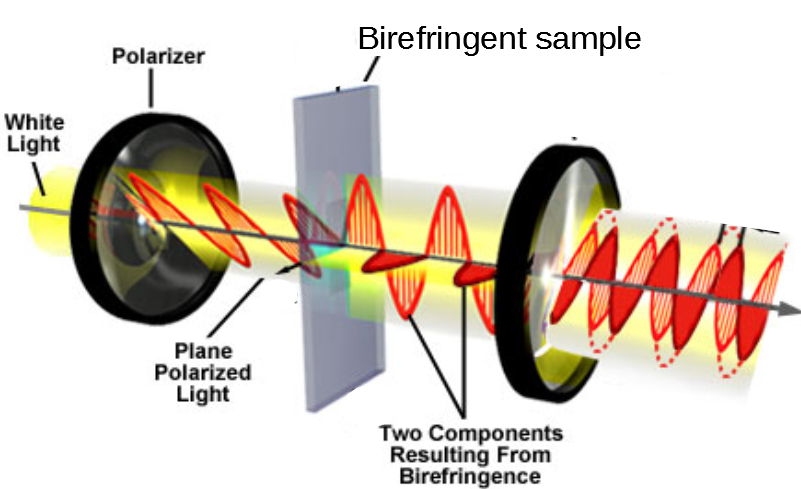
\includegraphics[width=8cm]{afbeeldingen/bf_principle.png}
	\caption{Schematic diagram of birefringence between two crossed polarizing windows. This figure was adapted from \cite{olympus}.}
	\label{fig_bf_diagram}
\end{figure}
	

\subsection{Error calculation}

If $Y$ is a variable which is a function of $A$,$B$,$C$, ... Then the error of $Y$, $u(Y)$, is given by equation \ref{eq_error}.

\begin{equation}
	\label{eq_error}
	u(Y) = \sqrt{\left(u(A) \frac{\partial Y}{\partial A}\right)^2 + \left(u(B) \frac{\partial Y}{\partial B}\right)^2 + \left(u(C) \frac{\partial Y}{\partial C}\right)^2 + ...}
\end{equation}

From this it follows that $u(d_{physical})$, $u(A)$ and $u(\Delta n)$, are given respectively by equations \ref{eq_u_d}, \ref{eq_u_A} and \ref{eq_u_bf}.

\begin{equation}
	\label{eq_u_d}
	u(d_{physical}) = \sqrt{\left( u(l_{pixel}) \cdot n_{pixels} \right)^2 + \left( u(n_{pixels}) \cdot l_{pixel} \right)^2}
\end{equation}

\begin{equation}
	\label{eq_u_A}
	u(A) = 1/4 \cdot \pi  \sqrt{(u(a) \cdot b)^2 + (u(b) \cdot a)^2}
\end{equation}

\begin{equation}
	\label{eq_u_bf}
	u(\Delta n) = \sqrt{\left( u(\Delta l_{path}) \cdot \frac{1}{D}\right)^2 + \left( u(D) \cdot \frac{l_{path}}{D^2}\right)^2}
\end{equation}















\begin{comment}
In  theTheorie  (Theory)  chapter,  you  describe  all  (and  only!)  the  theory needed  to  understand  and  interpret the experiments  in  the  remainder  of  the  report.    Explain  to  the  reader  why  a  piece  of  theory  is  relevant  for  your  research.  Equations  should  be  numbered.  If  an  equation  cannot  be  assumed  to  be  generally known by the readers (see General Hint 2 for the level of the audience), you should provide a reference to an accessible textbook or article (so not to the RP manual, lecture notes, Wikipedia etc.). In general, try to avoid referring to websites, online data or Wikipedia.
\end{comment}